\documentclass[french]{beamer}
\graphicspath{{figures/}}
\usepackage[utf8]{inputenc}
\usepackage[T1]{fontenc}
\usepackage{lmodern}
\usepackage{amsmath, amssymb}

\usepackage{babel}


%CHOIX DU THEME et/ou DE SA COULEUR
% => essayer différents thèmes (en décommantant une des trois lignes suivantes)
\usetheme{Hannover}
%\usetheme{Madrid}
%\usetheme{Copenhagen}

% => il est possible, pour un thème donné, de modifier seulement la couleur
%\usecolortheme{crane}
%\usecolortheme{seahorse}

%\useoutertheme[left]{sidebar}


%Pour le TITLEPAGE
\title{Stage chez Teamber - Développement de fonctionnalités}

\author[Antoine Perrot]{Antoine PERROT}

\date{du 27 avril au 31 juillet 2020}
\institute[UT3 -- FSI]{Université Toulouse~3 -- Faculté des sciences et ingénierie}


\begin{document}


\begin{frame}
	\titlepage
\end{frame}


\section*{Sommaire}
\begin{frame}{Sommaire}
	\tableofcontents
\end{frame}


\section{Optimisation de la répartition des tâches}
\begin{frame}{Optimisation de la répartition des tâches}
\begin{block}{Objectif :}
Répartir le travail intelligemment entre les utilisateurs en respectant un certain nombre de contraintes.
\end{block}
\end{frame}

\begin{frame}{Formulation du problème}
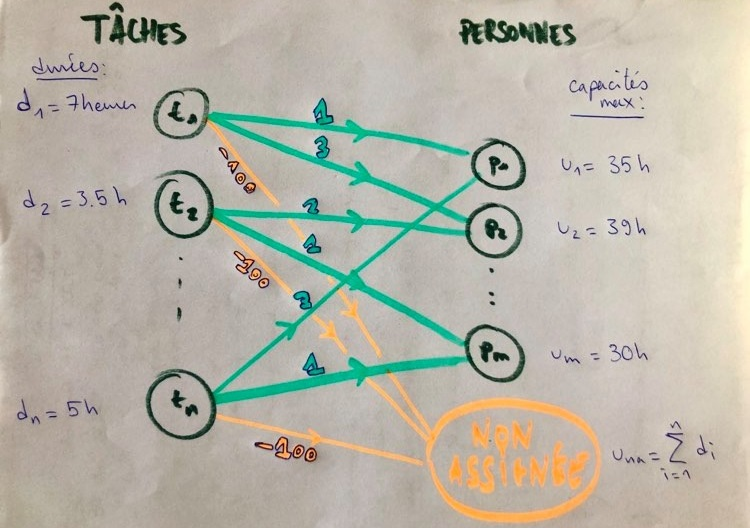
\includegraphics[width=0.9\textwidth>]{graphe}
\end{frame}

\begin{frame}
\begin{block}{Quantité à maximiser :}
L'utilité totale :
\[
\sum_{(i,j) \in \mathcal{A}} x_{ij}f_{ij} 
\]

\end{block}
\begin{block}{Sous les contraintes :}
\begin{itemize}
\item Distribution de toutes les heures :
\[
\forall i = 1,...,n  \sum_{j| (i,j) \in \mathcal{A}} x_{ij} = d_i
\]
\item Respect des capacités de travail :
\[
\forall j = 1,...,m  \sum_{i| (i,j) \in \mathcal{A}} x_{ij} \leq u_j
\]
\item Positivité :
\[
\forall (i,j) \in \mathcal{A},\; x_{ij} \geq 0
\]
\end{itemize}
\end{block}
\end{frame}

\begin{frame}
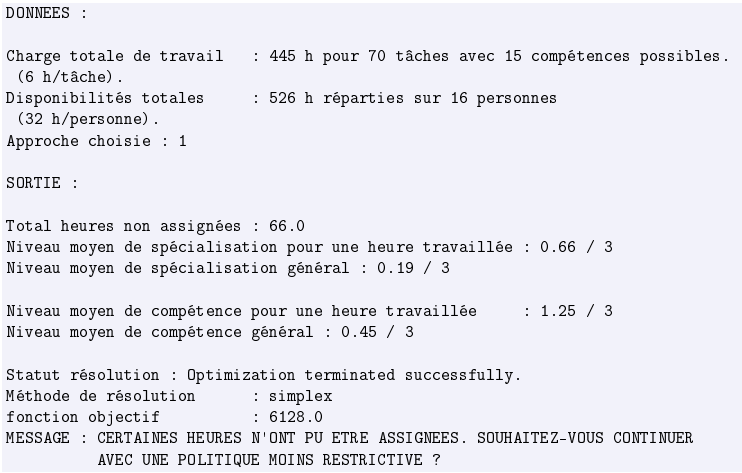
\includegraphics[width=0.9\textwidth>]{oadt1}
\end{frame}


\section{Optimisation des emplois du temps}
\begin{frame}{Optimisation des emplois du temps}
\begin{block}{But}
Suggérer des emplois du temps tenant compte des attentes des utilisateurs.
\end{block}
\end{frame}

\begin{frame}
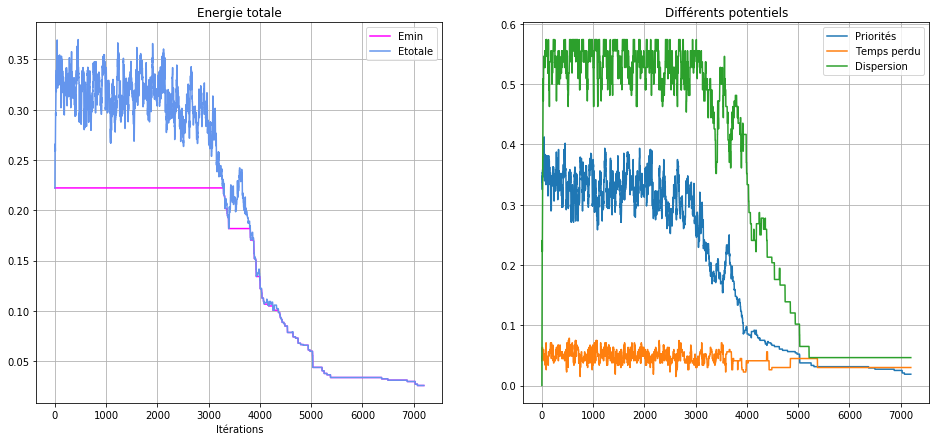
\includegraphics[width=0.9\textwidth>]{oedt1}
\end{frame}


\begin{frame}
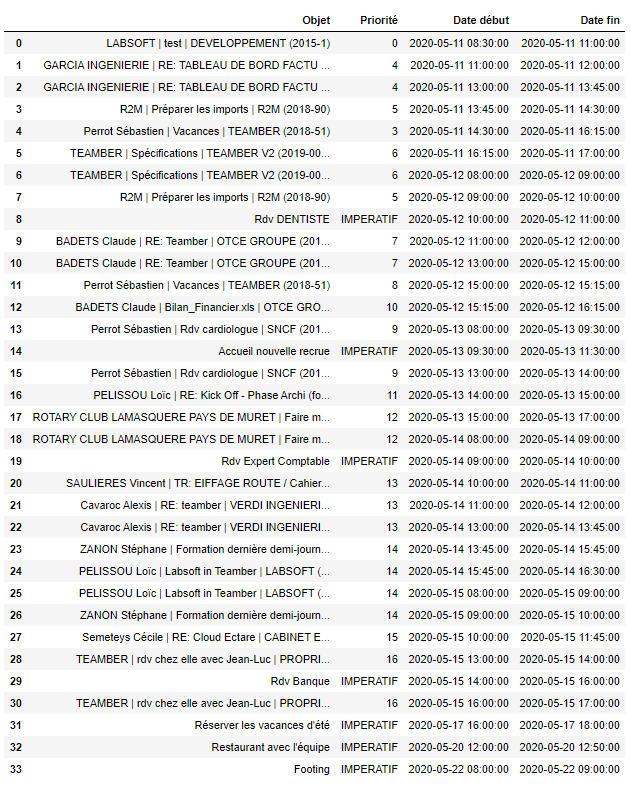
\includegraphics[width=0.9\textwidth>]{oedt2}
\end{frame}

\section{Complétion intelligente des tournées commerciales}
\begin{frame}{Complétion intelligente des tournées commerciales}
\begin{block}{But}
Ajouter intelligemment des points de passages à une tournée commerciale.
\end{block}
\end{frame}


\begin{frame}
\begin{block}{Tournée initiale}
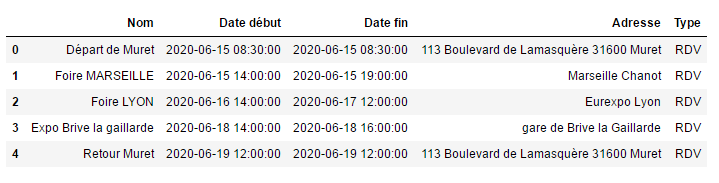
\includegraphics[width=0.9\textwidth>]{dfrdv}
\end{block}
\end{frame}


\begin{frame}
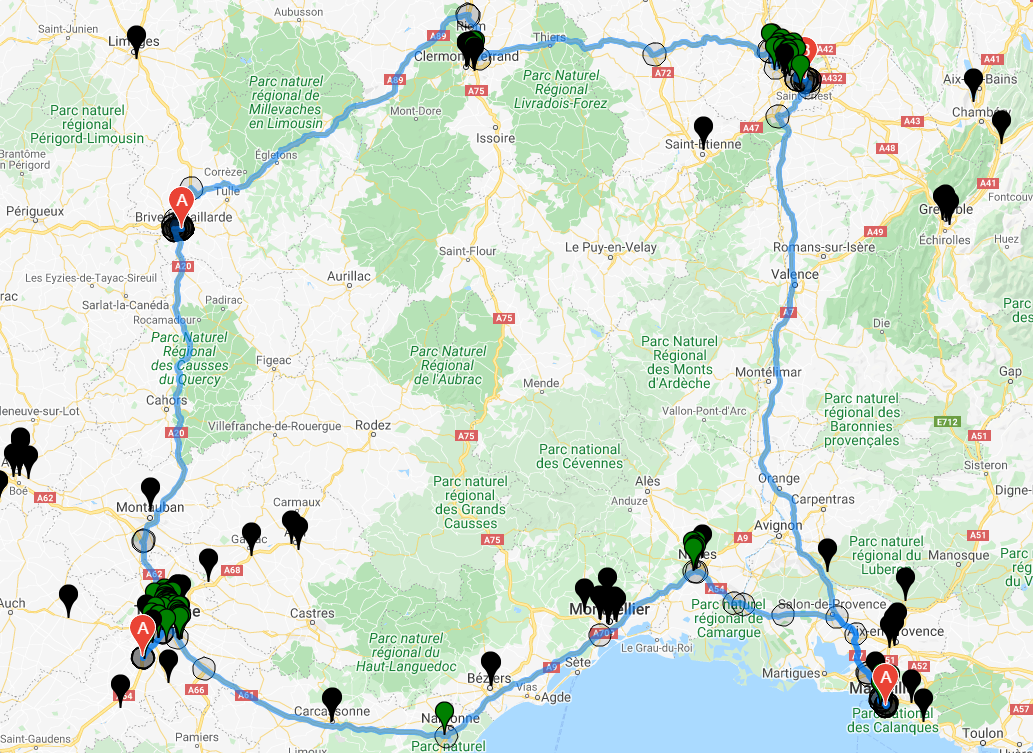
\includegraphics[width=0.9\textwidth>]{Circles2}
\end{frame}

\begin{frame}
\begin{block}{Tournée initiale}
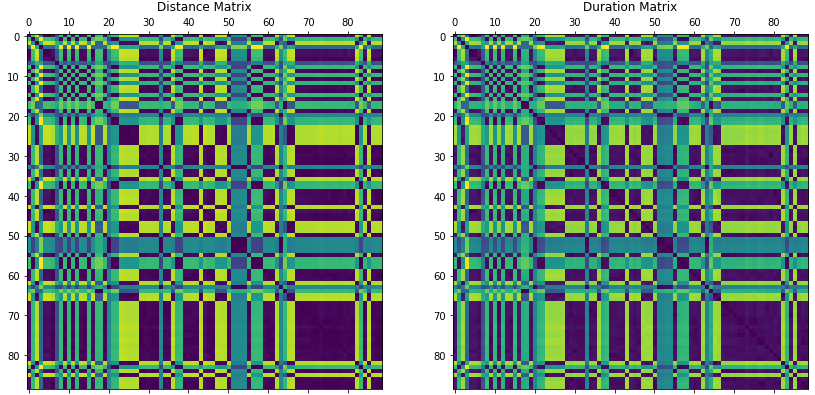
\includegraphics[width=0.9\textwidth>]{distance matrix}
\end{block}
\end{frame}

\begin{frame}
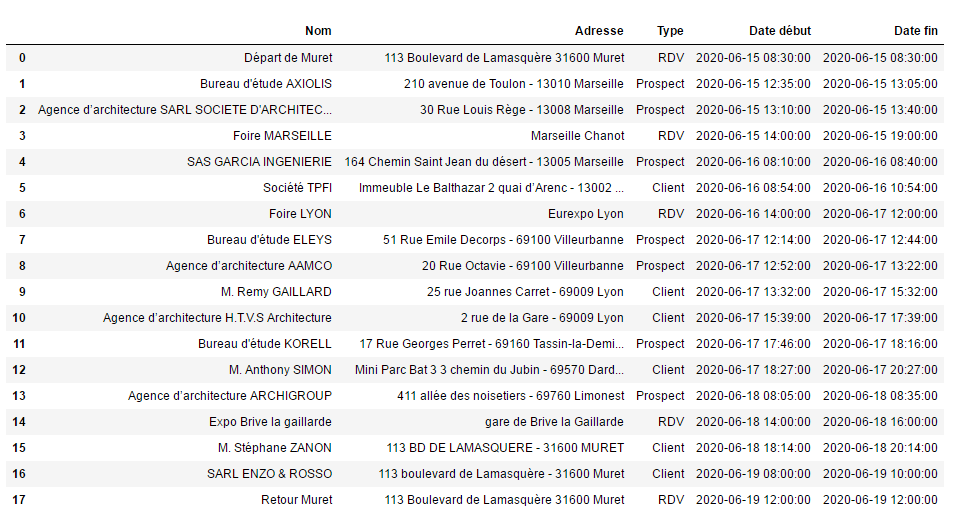
\includegraphics[width=0.9\textwidth>]{completion programme}
\end{frame}
\begin{frame}
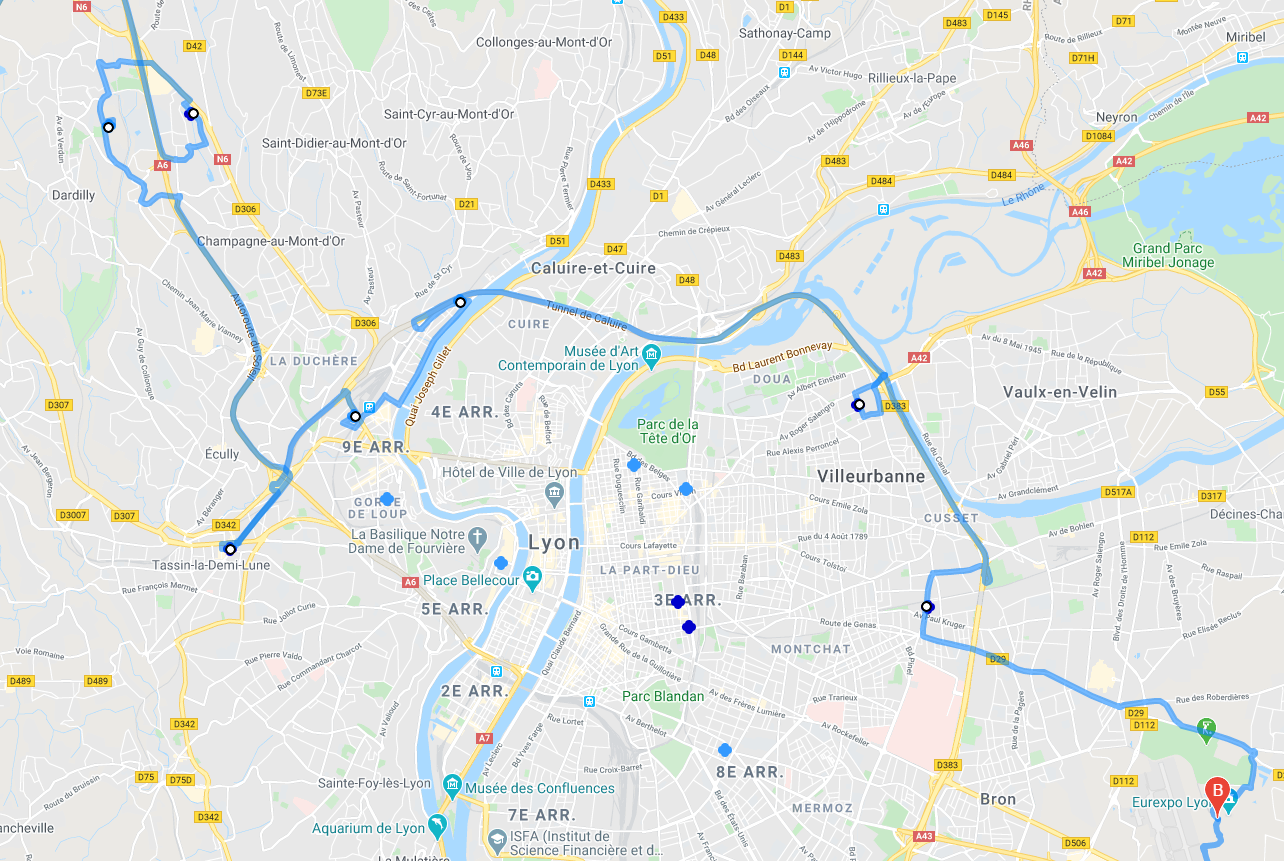
\includegraphics[width=0.9\textwidth>]{completion lyon}
\end{frame}


\end{document}
